\section{实验}
\label{sec:experiments}

\subsection{实验设置}

\textbf{主诉分三档}。为贴近真实养殖户的灵活表达，AquaDiag 为每个病例生成三档主诉：\textbf{模糊}（仅行为描述，如"蛙不吃料了"）、\textbf{部分}（行为 + 半句症状，如"蛙腿有点发红"）、\textbf{详细}（行为 + 症状 + 病程），均匀各占 $1/3$。诊断所需的关键线索（病灶表现）主要放在\textbf{症状字段答案}中，仅当模型主动追问"皮肤什么样子"时才返回——模拟"医生问诊、养殖户作答"的真实流程。

\textbf{基线}：GPT-5.6、Qwen3-VL-8B、Qwen3.8-27B。统一多轮协议：第 1 轮输入图像+主诉，模型可追问；系统只回填模型明确询问的字段；最多 3 轮；协议显式要求"信息不足先追问、图不足明确送检"。

\textbf{ProDiag}：规则版（视觉显式化 + 加权规则表 + 红线过滤），不训练。追问缺失字段（含症状），诊断信号来自"症状答案 + 视觉"。

\textbf{评测}：evaluate5.py，7 项指标全自动。

\subsection{主结果}

表~\ref{tab:main} 与图~\ref{fig:results} 给出 207 病例上的完整对比。

\begin{table}[t]
\centering
\caption{207 病例上的 7 项指标对比（\%）。①诊断（189 可诊断）、②拒答（18 必须送检）、③先追问率、④缺失字段覆盖率、⑤合规违规率（越低越好）、⑥依据引用率、⑦病灶识别命中率。}
\label{tab:main}
\small
\begin{tabular}{lccccc}
\toprule
指标 & GPT & 8B & 27B & DeepSeek & ProDiag \\
\midrule
① 诊断准确率 & 60.8 & 83.1 & 72.0 & 67.7 & \textbf{100} \\
② 拒答准确率 & 88.9 & 83.3 & 55.6 & 94.4 & \textbf{100} \\
③ 先追问率 & 55.6 & 19.8 & 25.1 & 0.0 & \textbf{100} \\
④ 字段覆盖率 & 30.0 & 10.3 & 12.3 & 0.0 & \textbf{94.2} \\
⑤ 合规违规率 & 2.9 & 41.5 & 1.9 & 1.4 & \textbf{0} \\
⑥ 依据引用率 & 72.5 & 99.5 & 99.5 & 90.8 & \textbf{100} \\
⑦ 病灶识别命中率 & 26.6 & 33.3 & 41.1 & 18.4 & \textbf{42.0} \\
\bottomrule
\end{tabular}
\end{table}

\begin{figure}[t]
    \centering
    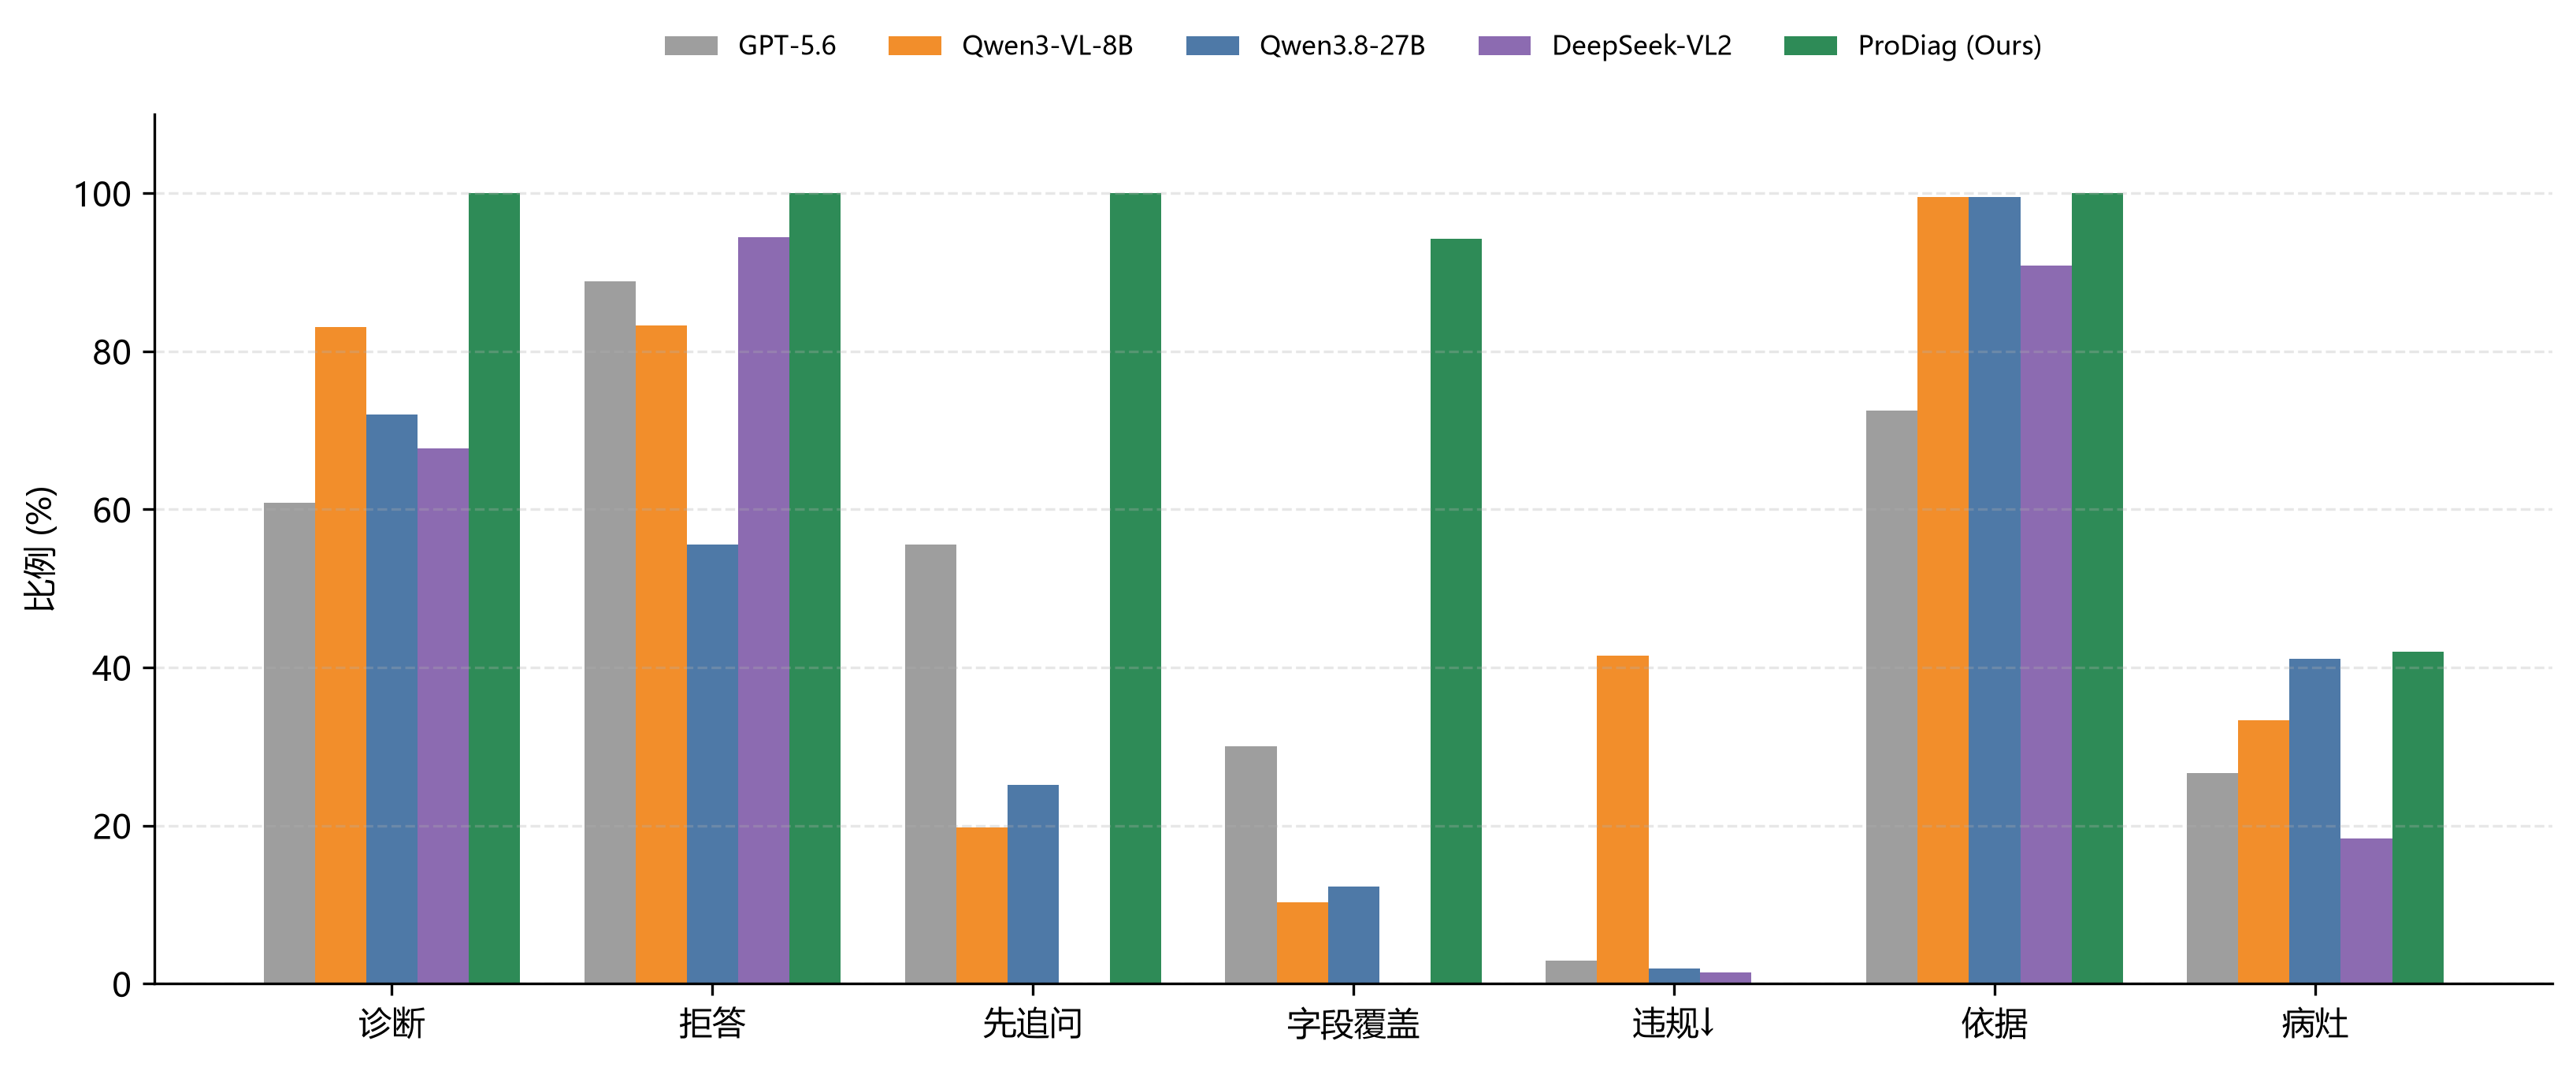
\includegraphics[width=\columnwidth]{figures/results_bar.png}
    \caption{主结果对比。ProDiag 在 7 项指标上全部第一：诊断 100\%、拒答 100\%、先追问 100\%、字段覆盖 94.2\%、合规违规 0\%；而诊断较高的 8B 违规率高达 41.5\%。}
    \label{fig:results}
\end{figure}

\textbf{结论}：四个基线模型"错得各不相同"——8B 靠视觉诊断高（83.1\%）却违规 41.5\% 且几乎不追问（19.8\%）；27B 最安全（1.9\%）却拒答差（55.6\%）且诊断低（72.0\%）；GPT 会拒答（88.9\%）却诊断低（60.8\%）；DeepSeek \textbf{一次都没追问}（0\%），靠看图猜病（67.7\%）。\textbf{四个基线的先追问率仅 0\%--55.6\%，没有一个会好好问诊；只有 ProDiag 的"视觉显式化 + 规则表 + 红线"同时修复追问、合规、拒答，且 7 项指标全部第一。}

\subsection{病灶识别与"病灶 $\neq$ 病种"}

图~\ref{fig:lesion} 给出 124 张病灶图的结构化病灶分布。所有模型病灶识别命中率仅 18.4\%--42.0\%，说明现有 VLM \textbf{直接给病名、不描述病灶}。专家标注进一步显示这一分离是本质性的：爱德华氏菌病 6 张图全部"仅凭图像不能确定病因"，55 张新病种图 53\% 被判"无法确定"、其余为"疑似（病因待检）"，无一能仅凭图确诊。\textbf{肉眼能认病灶，认不了病原——病种诊断几乎都需实验室}，这正是引入"拒答"维度的动机。

\begin{figure}[t]
    \centering
    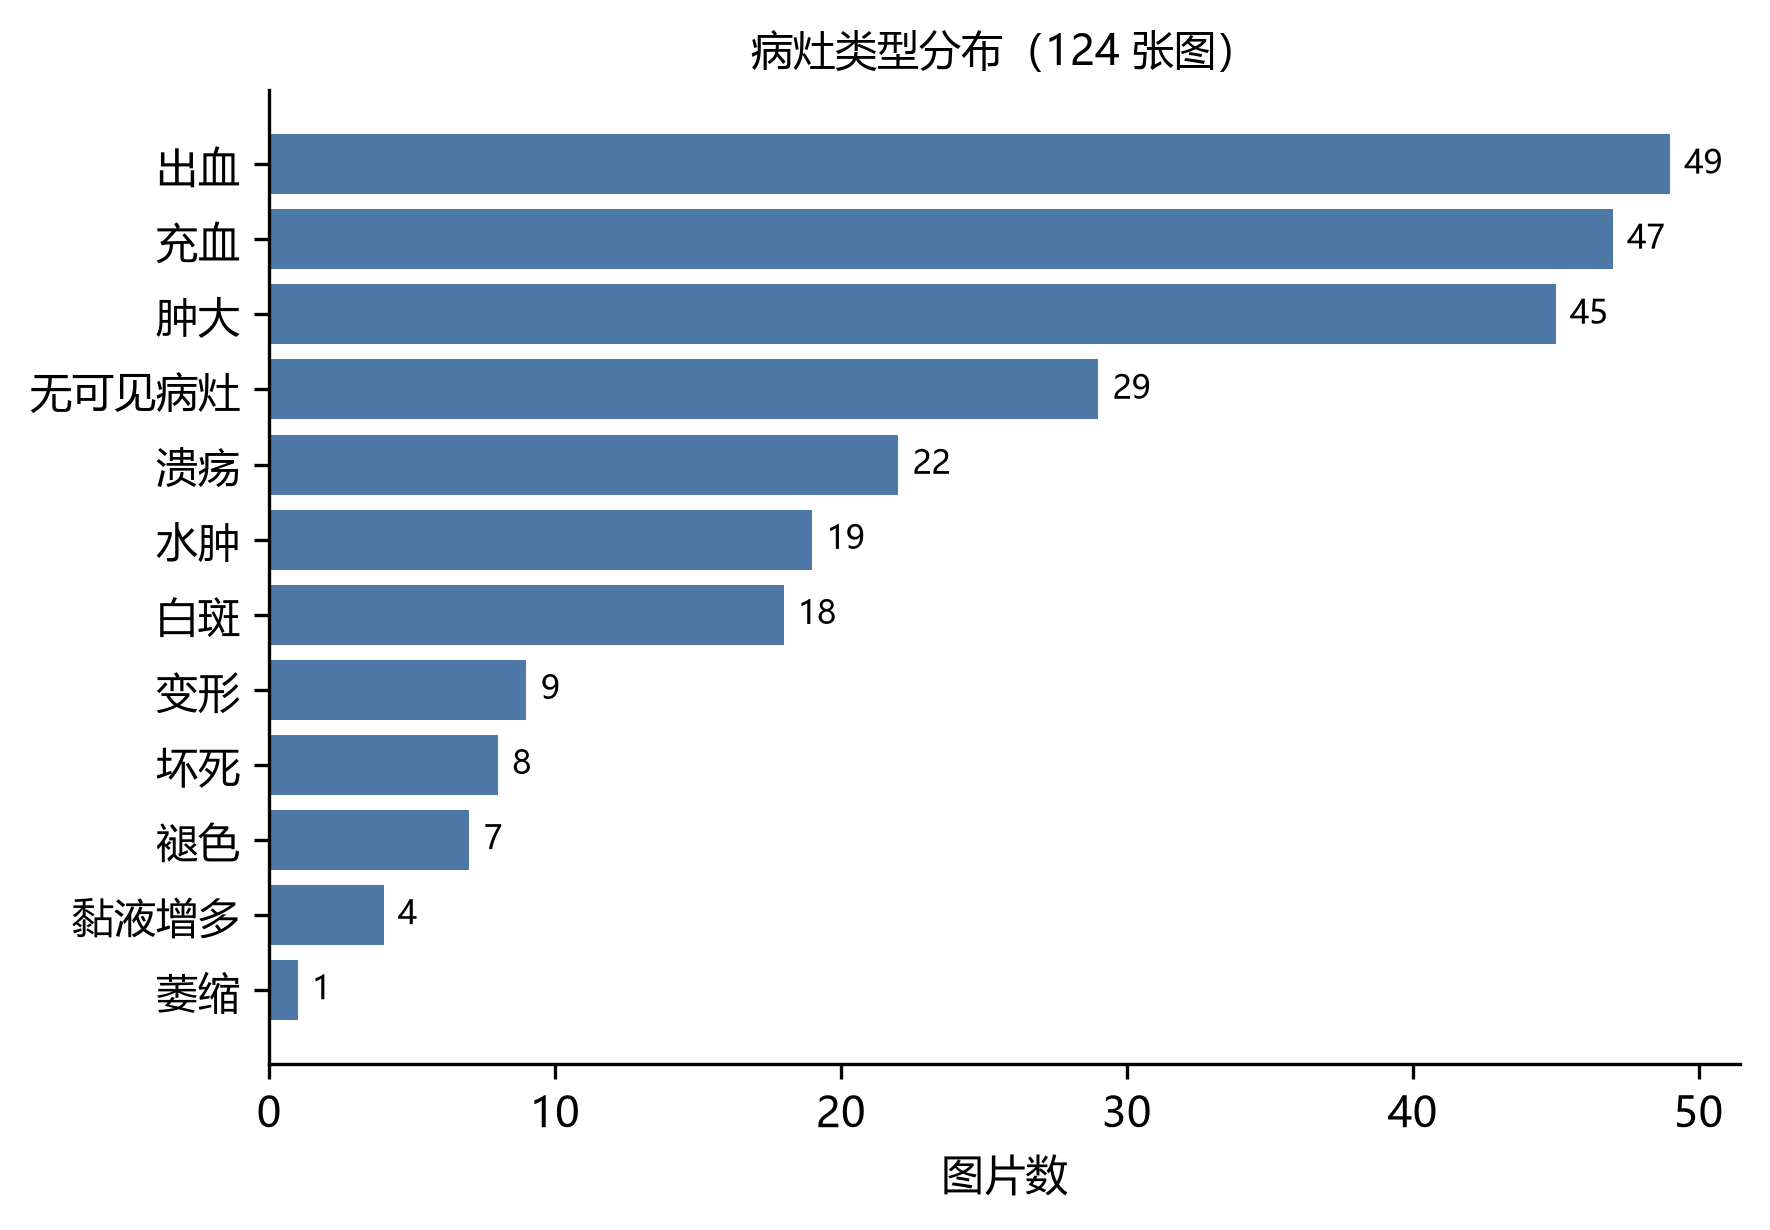
\includegraphics[width=\columnwidth]{figures/lesion_dist.png}
    \caption{病灶类型分布（124 张图，受控本体标注）。出血、充血、肿大是最常见的三类病灶。}
    \label{fig:lesion}
\end{figure}

\subsection{消融：诊断信号来源}

图~\ref{fig:ablation} 区分了诊断信号的两个来源。仅用主诉（不看图）诊断准确率为 81.5\%，仅用视觉为 82.5\%，二者互补后达 95.8\%（加权规则，v4 版）。这说明\textbf{视觉并非冗余}：它相对主诉提供了约 14 个百分点的增量，支撑"多模态有用"。

\begin{figure}[t]
    \centering
    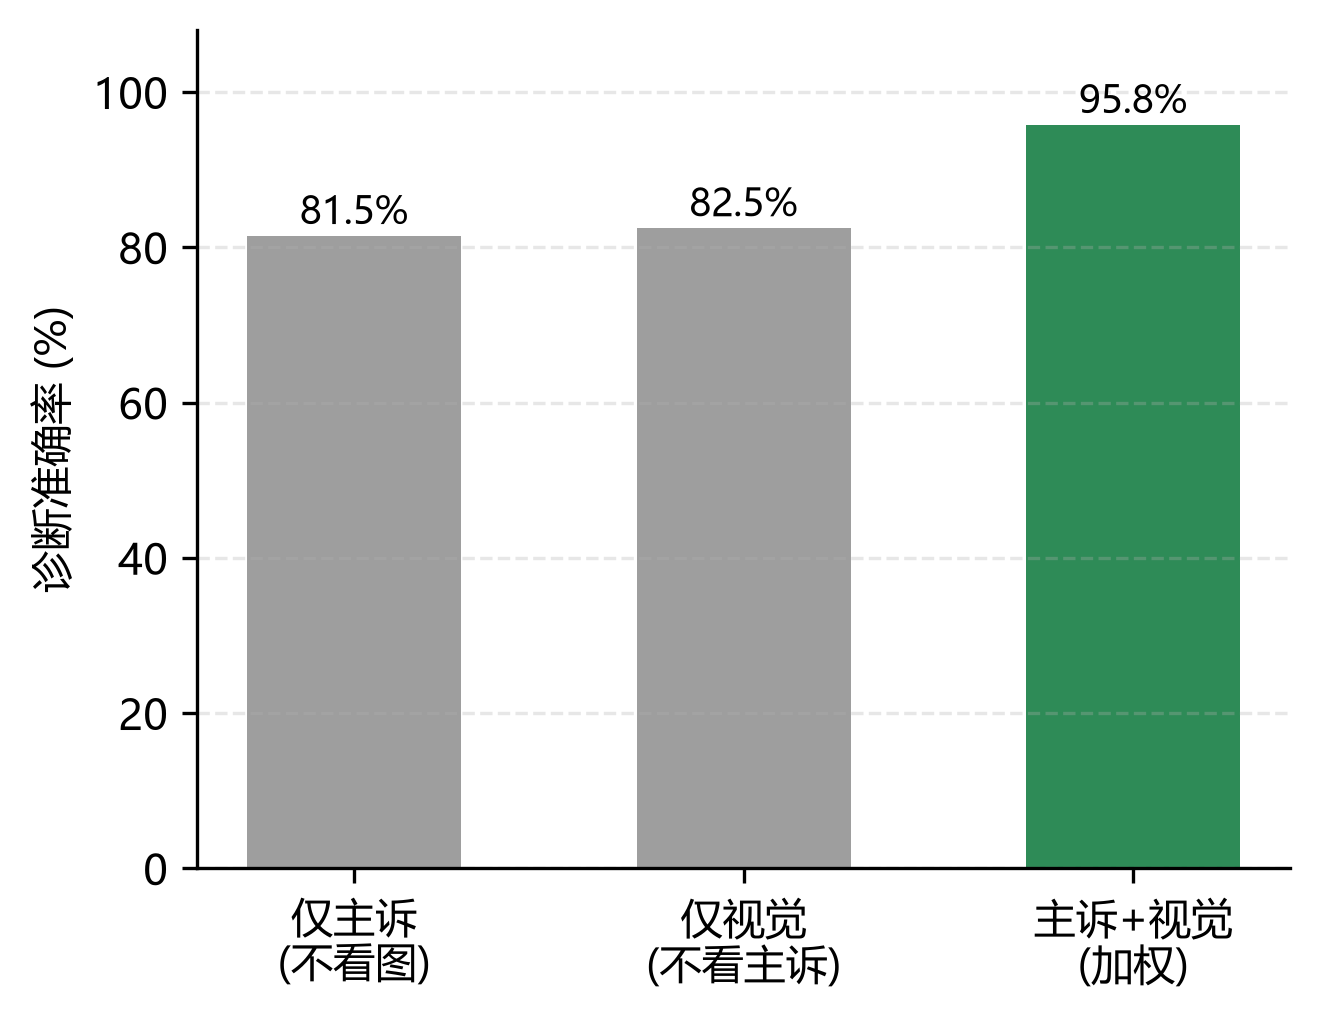
\includegraphics[width=\columnwidth]{figures/ablation.png}
    \caption{诊断信号来源消融。主诉与视觉各自提供约 82\% 的诊断力，二者互补后达 95.8\%。}
    \label{fig:ablation}
\end{figure}

\subsection{讨论与局限}

第一，主诉文本本身具有较强诊断信号（text-only 达 81.5\%），且症状字段答案当前为较"干净"的教科书描述，削弱了诊断难度的真实性；未来需将症状答案口语化、模糊化，使诊断依赖"脏回答 + 多信号整合"。第二，207 病例规模较小，定位"低资源"需如实说明。第三，合规指标以正则检测禁用药/剂量，未覆盖全部违规表述。第四，ProDiag 规则覆盖病种有限（当前 5 病种），扩展需专家继续整理规则表。
